\documentclass[onecolumn]{article}
\usepackage{graphicx}
\usepackage{float}
\restylefloat{figure}
\begin{document}

\title{The Sieve of Eratosthenes}

\author{Arjen Markus}

\maketitle

\section*{Introduction}
The Sieve of Eratosthenes is a remarkable elegant device to find all prime numbers in a certain range starting from 2:

\begin{itemize}
\item   Select the numbers 2 to N.
\item   Since 2 is a prime, we have our first result and we eliminate all multiples of 2 from the above set.
\item   The smallest one is again a prime and now we eliminate all multiples of that prime.
\item   Continue this way until all numbers have been eliminated.
\item   The numbers we used for this elimination process are the primes in the range 2 to N.
\end{itemize}

I was reminded of this algorithm by an article by Melissa O'Neill on its implementation in Haskell, one of the better known functional languages \cite{SieveEratosthenes}. Functional languages typically use compact recursive algorithms:

\begin{verbatim}
    primes = sieve [2..]

    sieve (p : xs) = p : sieve [x | x <- xs, x 'mod' p > 0]
\end{verbatim}

I wondered what solutions you can construct in Fortran in the way of compactness of code and memory use - as the latter is one of the themes in the article (another theme is whether Haskell code such as the above is truly an implementation of the Sieve). So let us examine how much memory is required and how much time is involved for a small variety of implementations.

\section*{Implementations in Fortran}

First consider this straightforward, iterative, implementation:

\begin{verbatim}
subroutine sieve( number, result )

    integer, intent(in)                :: number
    integer, dimension(:), allocatable :: result

    integer, dimension(:), allocatable :: array
    integer, dimension(:), allocatable :: primes
    integer, dimension(1)              :: p
    integer                            :: count

    allocate( array(number), primes(number) )

    array    = 1
    array(1) = 0
    primes   = 0

    count = 0
    do while ( any( array == 1 ) )
        p                 = maxloc( array )
        count             = count + 1
        primes(count)     = p(1)
        array(p(1)::p(1)) = 0
    enddo

    allocate( result(count) )
    result = primes(1:count)

end subroutine sieve
\end{verbatim}

The memory usage is clear: two arrays of $N$ elements are used and in the final step we need an array to store the
results, a total of $2N + N/\ln(N)$ (using a simple estimate for the number of primes lower than $N$).
We could get it down to $N + N/ln(N)$ elements by reusing the first elements of the array array as there are
always less primes than general integers.

The time necessary for this implementation can be expressed as the total number of array elements that are accessed. Per iteration we have:

\begin{itemize}
\item   The \verb+any()+ function will access at least the first $P$ elements (where $P$ is the prime to be found\footnote{We also assume that no temporary mask array is built}).
\item   The \verb+maxloc()+ function needs to iterate over the whole array.
\item   The last statement in the loop sets all multiples of the found prime to zero. It will do so without regard to values that may already have been set to zero.
\end{itemize}

The result per iteration is: $P + N + N/P$. Following O'Neill we estimate the total amount of work to be:

\begin{equation}
   \sum_{i=1}^{\pi(N)} (p_i + N + N/p_i) = \frac{1}{2} N \ln N + N^2 / {\ln N} + N \ln \ln N + O(N)
\end{equation}


where we have used the estimate that the i$^{th}$ prime is roughly i ln i, and sums can be replaced by integrals.
This is much more than the nominal time $N \ln \ln N$, that the true sieve requires.

A recursive implementation allows us to build up the array of results as we iterate (note the automatic
reallocation when we store the result):

\begin{verbatim}
subroutine sieve( number, result )

    integer, intent(in)                :: number
    integer, dimension(:), allocatable :: result

    integer, dimension(0)              :: work
    integer, dimension(:), allocatable :: array
    integer                            :: prime

    allocate( array(number) )

    array    = 1
    array(1) = 0
    prime    = 2

    call sieve_recursive( array, prime, work )
contains
recursive subroutine sieve3_recursive( array, prime, primes )
    integer, dimension(:) :: array
    integer               :: prime
    integer, dimension(:) :: primes

    integer, dimension(1) :: p

    p     = maxloc( array )
    prime = p(1)
    if ( array(prime) /= 0 ) then
        array(prime::prime) = 0
        call sieve_recursive( array, prime, [primes, prime] )
    else
        result = primes
    endif
end subroutine sieve_recursive
end subroutine sieve
\end{verbatim}

The memory we need for this implementation is larger than for the first implementation,
as we build up the array (the argument work) and intermediate arrays can only be deallocated
when the recursive subroutine that is doing the actual job returns. The accumulated memory for
this array is $N^2 \ln N / 2 + O(N)$. The time required for the computation, as measured in the number
of array elements being accessed, is roughly the same.

The troublesome element is, of course, searching for the next candidate via the \verb+maxloc()+ function.
This has to be done by scanning the entire array, yielding the $N^2 \ln N$ term in the above equation.

We can use a different tactic -- by storing all the candidates in the work array and removing the composite ones we find:

\begin{verbatim}
subroutine sieve( number, result )

    integer, intent(in)                :: number
    integer, dimension(:), allocatable :: result

    integer, dimension(:), allocatable :: array
    integer                            :: i

    array = [(i, i=2,number)]   ! Skip 1

    call sieve_recursive( [(i, i=1,0)], array )
contains
recursive subroutine sieve_recursive( primes, array )
    integer, dimension(:) :: primes
    integer, dimension(:) :: array

    if ( size(array) /= 0 ) then
        call sieve2_recursive( [primes, array(1)],  &
                 pack( array, mod(array, array(1)) /= 0 ) )
    else
        result = primes
    endif
end subroutine sieve_recursive
end subroutine sieve
\end{verbatim}

This is the most compact implementation sofar, but what about the memory usage and the computation time? This is more difficult to analyse as we have to know how the \verb+pack()+ function works. Assume the following algorithm:

\begin{itemize}
\item   First fill a temporary mask array with the result of the condition. While doing so, it counts the number of true values ($N'$ accesses, "true" count: $N' - N'/P$).
\item   Then allocate the result array and fill it (N' accesses, N' - N'/P elements in the result).
(where $N'$ is the number of elements left in the work array)
\end{itemize}

*** nader uit te werken ***

All of the above implementations have the drawback that you need to set the range of the integers to be examined. It is not possible to continue the work to find larger primes. That is taken care of by the last implementation:

\begin{verbatim}
subroutine sieve( next )
    integer, intent(out) :: next

    logical, save :: first = .true.

    integer, dimension(:), allocatable, save :: prime
    integer, dimension(:), allocatable, save :: multiple
    integer, dimension(:), allocatable       :: tmp
    integer                                  :: candidate

    if ( first ) then
        first = .false.
        prime    = (/ 2 /)
        multiple = (/ 2 /)
        next     = 2
        return
    endif

    !
    ! Regular search for the next one
    ! (Note: we need to update the multiples immediately)
    !
    candidate = minval(multiple) + 1
    do while ( any( multiple == candidate ) )
        candidate = candidate + 1
        do while ( any( multiple < candidate ) )
            multiple  = merge( multiple+prime, multiple, multiple < candidate )
        enddo
    enddo

    next = candidate

    prime    = (/ prime,    next /)
    multiple = (/ multiple, next /)
end subroutine sieve
\end{verbatim}

This version stores the primes found so far in a saved array prime, as well as the smallest multiple larger
than the last found prime. This allows it to start with the last prime and continue where it left off.
Analysing the computation time is more complicated than the other implementations.
The memory usage, however, is clear: all arrays (including any temporary that may be used by
the $merge()$ function) have as size the number of primes found sofar. To get an idea of the
computation time, let us instrument the routine and simply measure the number of array accesses
(under the simplifying assumption that the \verb+any()+ function examines the entire array).
The result is:

\begin{table}
\begin{center}
\begin{tabular}{rrr}
\hline
Index  & Prime  & Number of accesses \\
\hline
     1 &     3  &          5         \\
     2 &     5  &         20         \\
     3 &     7  &         20         \\
     4 &    11  &         50         \\
     5 &    13  &         32         \\
     6 &    17  &         74         \\
     7 &    19  &         44         \\
     8 &    23  &         98         \\
     9 &    29  &        164         \\
    10 &    31  &         62         \\
    11 &    37  &        200         \\
    12 &    41  &        146         \\
    13 &    43  &         80         \\
    14 &    47  &        170         \\
    15 &    53  &        272         \\
    16 &    59  &        290         \\
    17 &    61  &        104         \\
    18 &    67  &        326         \\
    19 &    71  &        230         \\
    20 &    73  &        122         \\
    21 &    79  &        380         \\
    22 &    83  &        266         \\
    23 &    89  &        416         \\
    24 &    97  &        578         \\
    25 &   101  &        302         \\
\hline
\end{tabular}
\end{center}
\end{table}

The somewhat surprising thing is that this is not at all monotonous function. For the first 1000 primes a plot of the prime versus the computation time gives:

\begin{figure}[h]
\begin{center}
\caption{Number of array accesses (estimate of the computation time) per prime.}
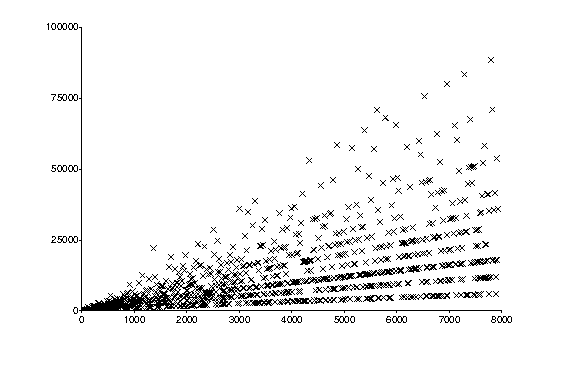
\includegraphics[width=0.95\textwidth]{computation_time.pdf}
\label{definition_sketch}
\end{center}
\end{figure}


Though the computation time (that is: the number of array accesses) is not completely accurately measured,
it would seem that the primes fall into different categories, each yielding a different, more or less linear
relationship between the prime and the computation time. It is not the purpose of this article to explore this
relationship any further, though.

The presented implementations differ widely: from a completely procedural approach to an almost functional one.
A remarkable aspect of the last implementation is that it does not use the elements of two arrays explicitly.
Instead it relies entirely on operations on the arrays as a whole.

\bibliography{eratosthenes}
\bibliographystyle{unsrt}
\end{document}

